\documentclass[letterpaper]{article}
\usepackage[top=2cm, bottom=3.5cm, left=2.5cm, right=2.5cm]{geometry}
\usepackage{amsmath,amsthm,amssymb}
% Indicator function
\usepackage{bbm}
\usepackage{tikz}
\usepackage{enumitem}
\usepackage{booktabs}
\usepackage[T1]{fontenc}
\usepackage{indentfirst}

\usepackage{graphicx}
\usepackage{epstopdf}

% Bold vectors and matrices
\renewcommand{\aa}{\mathbf{a}}
\providecommand{\xx}{\mathbf{x}}
\providecommand{\yy}{\mathbf{y}}
\providecommand{\1}{\mathbf{1}}
\providecommand{\0}{\mathbf{0}}
\providecommand{\mA}{\mathbf{A}}
\providecommand{\mI}{\mathbf{I}}

\providecommand{\lin}[1]{\ensuremath{\left\langle #1 \right\rangle}}
\providecommand{\norm}[1]{\ensuremath{\left\lVert#1\right\rVert}}

%
% The following macro is used to generate the header.
%
\newcommand{\homework}[4]{
   \thispagestyle{plain}
   \newpage
   \noindent
   \begin{center}
   \framebox{
      \vbox{\vspace{2mm}
    \hbox to 6.28in { {\bf EE-556: Mathematics of Data \hfill Fall 2019} }
       \vspace{6mm}
       \hbox to 6.28in { {\Large \hfill Homework \##1 - Due date: #2\hfill} }
       \vspace{4mm}
       \hbox to 6.28in { {\hfill Student: #3} }
      \vspace{2mm}}
   }
   \end{center}
}

\renewcommand{\phi}{\varphi}
\renewcommand{\epsilon}{\varepsilon}

% Use these for theorems, lemmas, proofs, etc.
\newtheorem{proposition}{Proposition}
\newtheorem{theorem}{Theorem}
\newtheorem{corollary}{Corollary}
\newtheorem{lemma}{Lemma}
\newtheorem{claim}{Claim}
\newtheorem{remark}{Remark}
\newtheorem{definition}{Definition}
\newtheorem{fact}{Fact}
\newtheorem{assumption}{Assumption}

\DeclareMathOperator*{\argmin}{arg\,min}
\DeclareMathOperator*{\argmax}{arg\,max}
\newcommand{\mbeq}{\overset{!}{=}}
\newcommand{\E}{\mathbb{E}}
\newcommand{\vect}[1]{\boldsymbol{#1}}

% Use Small capitals like in problem statement
\usepackage{sectsty}
\renewcommand{\thesection}{\Roman{section}} 
\renewcommand{\thesubsection}{\Roman{subsection}}
\allsectionsfont{\mdseries\scshape}

\begin{document}
\homework{1}{1\textsuperscript{st} November 2019}{Oriol Barbany Mayor}

\subsection*{Problem 1 - Geometric properties of the objective function $f$}
\begin{enumerate}[label=(\alph*)]
    \item By linearity of the gradient operator, we have that
    \begin{align}
        f(\xx, \mu) := \frac{1}{n}\sum_{i=1}^n g_i (\xx, \mu) + \frac{\lambda}{2}\norm{\xx}^2 \Longrightarrow \nabla f(\xx) = \frac{1}{n}\sum_{i=1}^n \nabla g_i (\xx, \mu) + \lambda \xx
    \end{align}
    
    \begin{align}
        \nabla g_i (\xx, \mu) = \begin{cases}
        -b_i \aa_i, & b_i \aa_i^T \xx \leq 0\\
        b_i \aa _i (b_i \aa_i^T \xx - 1), &0<b_i\aa_i^T \xx \leq 1 \\
        0,& 1\leq b_i \aa_i^T \xx
        \end{cases}
        \label{eq:1}
    \end{align}
    which yields
    
    \begin{align}
        \nabla f(\xx) = \frac{1}{n}\sum_{i=1}^n \left[ -b_i \aa_i\mathbbm{1}_{\{b_i \aa_i^T \xx  \leq 0\}} + b_i\aa _i (b_i\aa_i^T \xx -1 )\mathbbm{1}_{\{0<b_i \aa_i^T \xx\leq 1\}} \right] + \lambda \xx
        \label{eq:2}
    \end{align}
    
    Note that with the proposed notation, $\mI_L$ selects the coordinates that are in the linear region (first case of \eqref{eq:1}), and $\mI_Q$ the ones that lie in the quadratic region (second case). If we express \eqref{eq:2} in matrix form using $\tilde{\mA}$ as given in the problem description and the previous matrices, we get
    \begin{align}
        \nabla f(\xx) = - \frac{1}{n} \tilde{\mA} \mI_L \1 + \frac{1}{n} \tilde{\mA}^T \mI_Q [\tilde{\mA} \xx - \1] + \lambda \xx
    \end{align}
    
    Let's now compute the Lipschitz continuity constant of the gradient:
    \begin{align}
        \norm{\nabla f(\xx) - \nabla f(\yy)} &= \norm{\lambda (\xx - \yy) + \frac{1}{n}\tilde{\mA}^T \mI_Q\tilde{\mA} (\xx - \yy) - \frac{1}{n} \tilde{\mA} \mI_L \1 + \frac{1}{n} \tilde{\mA} \mI_L \1} \\
        &= \norm{\left( \lambda\mathbf{I} + \frac{1}{n}\tilde{\mA}^T \mI_Q\tilde{\mA} \right) (\xx - \yy)} \\
        &\leq \norm{\lambda\mathbf{I} + \frac{1}{n}\tilde{\mA}^T \mI_Q \tilde{\mA}} \norm{\xx - \yy}
    \end{align}
    where the inequality follows from definition of the spectral norm.
    
    Using the fact that $\lambda\mathbf{I} + \frac{1}{n}\tilde{\mA}^T \mI_Q \tilde{\mA} = \lambda\mathbf{I} + \frac{1}{n}\tilde{\mA}^T \tilde{\mA}$ given in the problem statement and using the triangle inequality, we get that
    \begin{align}
        \norm{\lambda\mathbf{I} + \frac{1}{n}\tilde{\mA}^T \mI_Q \tilde{\mA}} &:= \max_{\xx:\norm{\xx}=1} \norm{\left( \lambda\mathbf{I} + \frac{1}{n}\tilde{\mA}^T\mI_Q  \tilde{\mA} \right) \xx} \leq |\lambda| \max_{\xx:\norm{\xx}=1} \norm{\xx}  +\frac{1}{n} \max_{\xx:\norm{\xx}=1}  \norm{\tilde{\mA}^T \mI_Q \tilde{\mA}\xx} \\
        &:= \lambda + \frac{1}{n}\norm{\tilde{\mA}^T \tilde{\mA}} \leq \lambda + \frac{1}{n}\norm{\tilde{\mA}^T} \norm{\tilde{\mA}}
    \end{align}
    where the last inequality again follows from definition of the spectral norm and I assume that $\lambda$ is non-negative. The proof is completed using the fact that $\norm{\tilde{\mA}}=\norm{\mA}$ and $\norm{\tilde{\mA}^T}=\norm{\mA^T}$.
    
    \item Assuming that all the samples lie in the quadratic region, i.e. $\mI_Q = \mathbb{I}$ and $\mI_L=\0$:
    \begin{align}
        \nabla f(\xx) = \frac{1}{n} \tilde{\mA}^T [\tilde{\mA} \xx - \1] + \lambda \xx
    \end{align}
    the gradient $\nabla f$ exists in all domain of $\xx$ and correspond to a linear function on $\xx$, which is infinitely differentiable. We then say that $f$ is twice differentiable (in fact infinitely differentiable and thus also twice), and its hessian corresponds to
    \begin{align}
        \nabla^2 f(\xx) = \frac{1}{n} \tilde{\mA}^T \tilde{\mA} + \lambda\mathbb{I}=\frac{1}{n}\mA^T \mA + \lambda\mathbb{I}
    \end{align}
    where the equality follows since $b_i^2 = 1 \ \forall i$, which implies that $\tilde{\mA}^T \tilde{\mA} = \mA^T \mA$.
    
    \item 
    \begin{lemma}
        A function $f$ is $\mu-$strongly convex iff $\nabla^2 f(\xx) \succeq \mu \mathbb{I}$
        \label{prop:1}
    \end{lemma}
    \begin{proof}
        As seen in lectures, $f$ is $\mu-$strongly convex iff $g(\xx):=f(\xx)-\frac{\lambda}{2}\norm{\xx}$ is convex, and hence if $\nabla^2g(\xx) \succeq 0$. The proposition follows by combining these two.
    \end{proof}
    
    Given that we have the hessian of $f$, we can use Lemma \ref{prop:1} to compute the strong convexity constant:
    \begin{align}
        \xx^T \nabla^2 f(\xx) \xx  = \lambda + \frac{1}{n}\xx^T\mA^T \mA \xx \geq \lambda := \mu \quad \forall \xx
    \end{align}
    where the inequality follows since $\mA^T \mA$ is positive semidefinite. This latter is true since we can define $\yy:=\mA \xx$ and $\norm{y} := \yy^T \yy := \xx^T\mA^T \mA \xx $ will be non-negative by definition of the norm.
\end{enumerate}

\subsection*{Problem 2 - First order methods for SVM}

\subsection*{Problem 3 - Stochastic Gradient methods for SVM}
\begin{enumerate}[label=(\alph*)]
    \item
    Since we choose each index $i_k$ uniformly at random from all the $n$ samples, we have that
    \begin{align}
        \E[\nabla f_{i_k}(\xx)] &= \frac{1}{n} \sum_{i=1}^{n} \nabla f_i(\xx) \\
        &= \lambda \xx + \frac{1}{n}\sum_{i=1}^n \left[ -b_i \aa_i\mathbbm{1}_{\{b_i \aa_i^T \xx  \leq 0\}} + \aa _i(\aa_i^T \xx - b_i )\mathbbm{1}_{\{0<b_i \aa_i^T \xx\leq 1\}} \right] \\
        &:= \nabla f(\xx)
    \end{align}
    where the last equality is the one already found in \eqref{eq:1}.
    
    \item
    \begin{assumption}
        Assume w.l.o.g. that sample $i_k$ lies in the quadratic region
        \label{as:1}
    \end{assumption}
    
    Taking Assumption \ref{as:1}, we have that
    \begin{align}
        \norm{\nabla f_{i_k}(\xx) - \nabla f_{i_k}(\yy)} = \norm{\lambda(\xx - \yy) + \aa_{i_k} \aa_{i_k}^T (\xx - \yy)} \leq \norm{\lambda\mathbb{I} + \aa_{i_k} \aa_{i_k}^T}\norm{\xx + \yy}
    \end{align}
    where the inequality follows by definition of the spectral norm.
    
    Using triangle inequality as in problem 1 gives
    \begin{align}
        \norm{\lambda\mathbb{I} + \aa_{i_k} \aa_{i_k}^T} &\leq \lambda + \norm{\aa_{i_k} \aa_{i_k}^T} := \lambda + \max_{\xx:\norm{\xx}=1} \norm{\aa_{i_k} \aa_{i_k}^T x} := \lambda + \max_{\xx:\norm{\xx}=1} \sqrt{x^T \aa_{i_k} \aa_{i_k} ^T \aa_{i_k} \aa_{i_k}^T x} \\
        &:=\lambda + \max_{\xx:\norm{\xx}=1} \sqrt{x^T \norm{\aa_{i_k}} ^2 \norm{\aa_{i_k}} ^2 x} = \lambda + \norm{\aa_{i_k}} ^2 \max_{\xx:\norm{\xx}=1} \norm{x} = \lambda + \norm{\aa_{i_k}} ^2
    \end{align}
    
    Note that assumption \ref{as:1} is w.l.o.g. since if we lie on the linear region,
    \begin{align}
        \norm{\nabla f_{i_k}(\xx) - \nabla f_{i_k}(\yy)} = \norm{\lambda(\xx - \yy)} = \lambda \norm{\xx-\yy} < L\norm{\xx-\yy}
    \end{align}
    hence global smoothness is the same (valid upper bound) even if it's not locally tight for the samples in the linear region.
    
\end{enumerate}

\begin{figure}
    \centering
    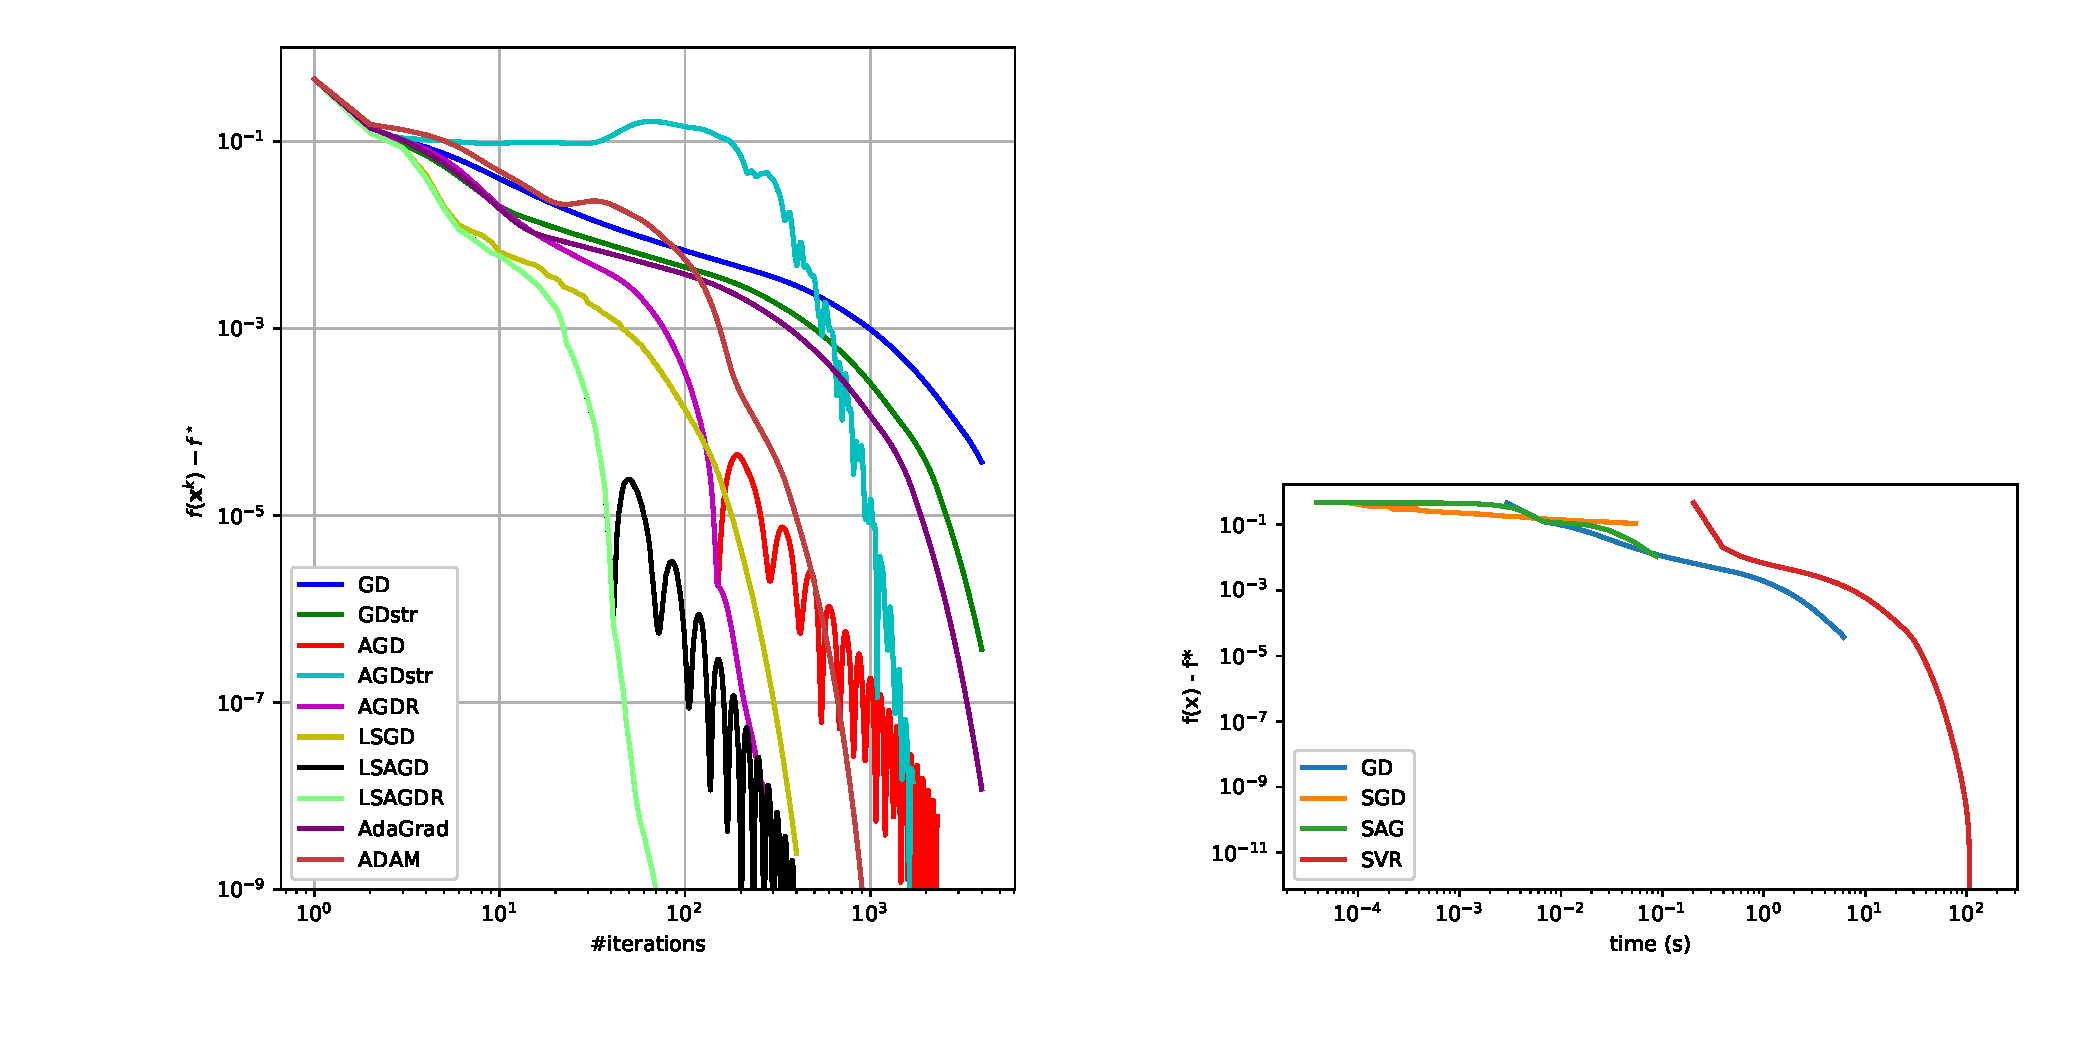
\includegraphics[scale=0.4]{Figure_1}
    \caption{Caption}
    \label{fig:my_label}
\end{figure}

\begin{itemize}
    \item Why do the algorithms in second graph start at different times?
    \item Emphasize Nesterov ripples and similarity of restart version until the first ripple.
    \item Compare algorithms also for the hyperparameters they use
    \item Can also do time analysis for first graph and iterations for second
\end{itemize}

\end{document}
